\documentclass[a4paper,12pt]{article}
%\documentclass[fleqn]{article}

% ---パッケージ---
\usepackage{amsmath,amssymb}    %数式用
\usepackage{tcolorbox}   %囲み枠用(tcolorboxに変更)
\usepackage{geometry}   %余白調節
\usepackage{tikz}  % ← 図を描くためのTikZパッケージ
\geometry{margin=25mm}  %余白を少し狭く
\usetikzlibrary{decorations.pathmorphing,patterns,positioning,arrows.meta} % バネ・壁の模様
\tikzset{
  block/.style = {draw, rectangle, minimum height=2em, minimum width=3em},
  sum/.style = {draw, circle, inner sep=0pt, minimum size=5mm},
  input/.style = {coordinate},
  output/.style = {coordinate}
}
\usetikzlibrary{calc}
\usepackage{pgfplots}  % ← 追加(グラフ用)
\pgfplotsset{compat=newest} % ← 推奨設定

% --- 日本語用パッケージ ---
\usepackage{luatexja}         % 日本語表示に必要
\usepackage{luatexja-fontspec} % フォント指定用

% --- フォント指定(Overleaf標準フォント)---
\setmainjfont{IPAexMincho}  % 明朝体
%\setmainjfont{IPAexGothic}  % ゴシック体にしたい場合

% --- tcolorbox の設定 ---
\tcbset{
    colframe=black,
    colback=white,         % 本文の背景(白)
    boxrule=0.8pt,
    arc=3pt,
    outer arc=3pt,
    boxsep=4pt,
    coltitle=black,
    colbacktitle=gray!20,  % タイトルの背景(グレー)
    fonttitle=\normalsize
}

\begin{document}
\noindent
\text{制御工学Ⅰ 演習② 解答}\\
\text{2025/06/11}\\
\text{Yudai}\\



% ---------------[1]--------------- 済

解説動画あるし作らないかも
後回し
1. 以下の式に関するラプラス逆変換を求めよ.
\[
    \renewcommand{\arraystretch}{3.0} % ← 行の高さ倍率を変更(1.0が標準)
    \begin{tabular}{@{}rl@{\quad\quad}rl@{}}
    (1) & $G_1(s) = \dfrac{4}{s+5}$                 & (2) & $G_2(s) = \dfrac{s+7}{s^2+2s+5}$ \\
    (3) & $G_3(s) = \dfrac{1}{s^3+11s^2+40s+48}$    & (4) & $G_4(s) = \dfrac{1}{Ts+1} \quad [Tは定数]$ \\
    (5) & $G_5(s) = \dfrac{1}{s(s+2)(s+3)^2}$       & (6) & $G_6(s) = \dfrac{1}{(s^2+1)(s^2+4)}$ \\
    \end{tabular}
    \]\\

\begin{tcolorbox}[title={1. (1) \( G_1(s)=\dfrac{4}{s+5} \)}]
    \quad 両辺にラプラス逆変換を施すと,
    \vspace{-3mm}
    \begin{align*}
        &\qquad \mathcal{L}^{-1} \left[ G_1(s) \right] 
        =\mathcal{L}^{-1} \left[ \frac{4}{s+5} \right] \\
        &\Leftrightarrow x(t) = 4 e^{-5t}
    \end{align*}
\end{tcolorbox}

\begin{tcolorbox}[title={1. (2) \( G_2(s)=\dfrac{ s + 7 }{ s^2 + 2s + 5} \)}]
    \vspace{-3mm}
  \begin{align*}
      &\qquad G_2(s) =\frac{ s + 7 }{ s^2 + 2s + 5}  \\
      &\Leftrightarrow G_2(s) =\frac{ (s + 1) + 6 }{ ( s + 1 )^2+ 2^2} \\
      &\Leftrightarrow G_2(s) 
      = \frac{ (s + 1) }{ ( s + 1 )^2+ 2^2}
      + \frac{ 6 }{ ( s + 1 )^2+ 2^2} 
  \end{align*}
  
  \quad 両辺にラプラス逆変換を施すと,
  \vspace{-3mm}
  \begin{align*}
      &\qquad \mathcal{L}^{-1} \left[ G_2(s) \right] 
      =\mathcal{L}^{-1} \left[ \frac{ (s + 1) }{ ( s + 1 )^2+ 2^2} \right]
      +\mathcal{L}^{-1} \left[ \frac{ 6  }{ ( s + 1 )^2+ 2^2} \right] \\
      &\Leftrightarrow g_2(t) = e^{-t} cos(2t) +3 e^{-t} sin(2t)
  \end{align*}
\end{tcolorbox}

\begin{tcolorbox}[title={1. (3) \( G_3(s)=\dfrac{ 1 }{ s^3 + 11 s^2+ 40s + 48 } \) }]
    \vspace{-3mm}
  \begin{align*}
      &\qquad G_3(s) =\frac{ 1 }{ s^3 + 11 s^2+ 40s + 48 }  \\
      &\Leftrightarrow G_3(s) =\frac{ 1 }{ (s+3)(s+4)^2 }  \\
      &\Leftrightarrow G_3(s) 
      = \frac{1}{s+3}
      + \frac{-1}{s + 4}
      + \frac{-1}{(s + 4)^2}
      \quad [\because ヘヴィサイドの展開定理]
  \end{align*}
  
  \quad 両辺にラプラス逆変換を施すと,
  \vspace{-3mm}
  \begin{align*}
      &\qquad \mathcal{L}^{-1} \left[ G_3(s) \right] 
      =\mathcal{L}^{-1} \left[ \frac{1}{s+3} \right]
      +\mathcal{L}^{-1} \left[ \frac{-1}{s + 4} \right]
      +\mathcal{L}^{-1} \left[ \frac{-1}{(s + 4)^2} \right] \\
      &\Leftrightarrow g_3(t) = e^{-3t} - e^{-4t} - te^{-4t}
  \end{align*}
\end{tcolorbox}

\begin{tcolorbox}[title={1. (4) \( G_4(s)=\dfrac{1}{Ts+1} \)}]
    \begin{align*}
        &\qquad G_4(s) =\frac{1}{Ts+1}  \\
        &\Leftrightarrow G_4(s) =\frac{(\frac{1}{T})}{ s+(\frac{1}{T})} 
    \end{align*}
    \quad 両辺にラプラス逆変換を施すと,
    \vspace{-3mm}
    \begin{align*}
        &\qquad \mathcal{L}^{-1} \left[ G_4(s) \right] 
        =\mathcal{L}^{-1} \left[ \frac{(\frac{1}{T})}{ s+(\frac{1}{T})} \right] \\
        &\Leftrightarrow g_4(t) = \frac{1}{T} e^{-\frac{t}{T}}
    \end{align*}
\end{tcolorbox}

\begin{tcolorbox}[title={1. (5) \( G_5(s)=\dfrac{ 1 }{ s ( s + 2 ) ( s + 3 )^2 } \) }]
    \vspace{-3mm}
  \begin{align*}
      &\qquad G_5(s) =\frac{ 1 }{ s ( s + 2 ) ( s + 3 )^2 }  \\
      &\Leftrightarrow G_5(s) 
      = \frac{\frac{1}{18}}{s}
      + \frac{(-\frac{1}{2})}{s + 2} 
      + \frac{\frac{1}{3}}{(s + 3)^2} 
      + \frac{\frac{4}{9}}{s + 3} 
  \end{align*}
  
  \quad 両辺にラプラス逆変換を施すと,
  \vspace{-3mm}
  \begin{align*}
      &\qquad \mathcal{L}^{-1} \left[ G_5(s) \right] 
      =\mathcal{L}^{-1} \left[ \frac{\frac{1}{18}}{s} \right]
      + \mathcal{L}^{-1} \left[ \frac{(-\frac{1}{2})}{s + 2} \right]
      + \mathcal{L}^{-1} \left[ \frac{\frac{1}{3}}{(s + 3)^2} \right]
      + \mathcal{L}^{-1} \left[ \frac{\frac{4}{9}}{s + 3} \right] \\
      &\Leftrightarrow g_5(t) = \frac{1}{18} - \frac{1}{2}e^{-2t} + \frac{1}{3}e^{-3t} +\frac{4}{9}e^{-3t}\\
      &\Leftrightarrow g_5(t) =\frac{1}{18} \left(1 - 9e^{-2t} + 8e^{-3t} +6te^{-3t} \right)
  \end{align*}
\end{tcolorbox}

\begin{tcolorbox}[title={1. (6) \( G_6(s)=\dfrac{ 1 }{ ( s^2 + 1 ) ( s^2 + 4 ) } \) }]
    \vspace{-3mm}
    \begin{align*}
      &\qquad G_6(s) =\frac{ 1 }{ ( s^2 + 1 ) ( s^2 + 4 ) } \\
      &\Leftrightarrow G_6(s) 
      = \frac{ \frac{1}{3} }{ ( s^2 + 1 ) }
      + \frac{ -\frac{1}{3} }{ ( s^2 + 4 ) }
  \end{align*}
  
  \quad 両辺にラプラス逆変換を施すと,
  \vspace{-3mm}
  \begin{align*}
      &\qquad \mathcal{L}^{-1} \left[ G_6(s) \right] 
      =\mathcal{L}^{-1} \left[ \frac{ \frac{1}{3} }{ ( s^2 + 1 ) } \right]
      +\mathcal{L}^{-1} \left[ \frac{- \frac{1}{3} }{ ( s^2 + 4 ) } \right] \\
      &\Leftrightarrow g_6(t) = \frac{1}{3}sin t -\frac{1}{6}sin 2t
  \end{align*}
  
\end{tcolorbox}
\newpage

% ---------------[2]---------------
\noindent
2.下図に示すシステムにおいて、システム全体の伝達関数を求めよ。なお、各伝達関数
\(G_i(s)\)については問1.の伝達関数を代入しないこと。
\vspace{2mm}

\begin{minipage}[t]{0.45\linewidth}
  (1)
  \begin{center}
    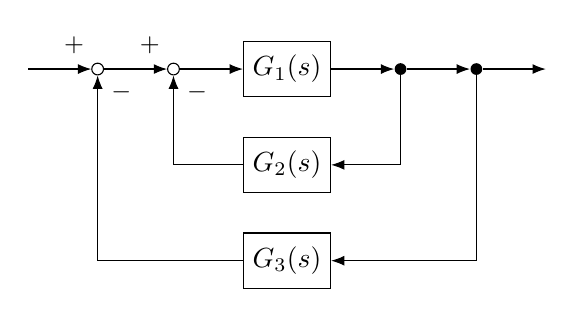
\begin{tikzpicture}[auto, node distance=0.8cm and 0.8cm, >=Latex]

      % --- 上段ノード ---
      \node[input] (input) {};
      \node[circle, draw, inner sep=1.5pt, right=of input] (sum1) {};           % 合流点①
      \node[circle, draw, inner sep=1.5pt, right=of sum1] (sum2) {}; % 合流点②
      \node[block, right=of sum2] (G1) {$G_1(s)$};              % G1
      \node[circle, fill=black, inner sep=1.5pt, right=of G1] (branch1) {}; % 分岐点①
      \node[circle, fill=black, inner sep=1.5pt, right=of branch1] (branch2) {}; % 分岐点②
      \node[output, right=of branch2] (output) {};
    
      % --- 下段ノード ---
      \node[block, below=0.5cm of G1] (G2) {$G_2(s)$};     % G2
      \node[block, below=0.5cm of G2] (G3) {$G_3(s)$};     % G3
    
      % --- 線描画 ---
      \draw[->] (input) -- (sum1);
      \draw[->] (sum1) -- (sum2);
      \draw[->] (sum2) -- (G1);
      \draw[->] (G1) -- (branch1);
      \draw[->] (branch1) -- (branch2);
      \draw[->] (branch2) -- (output);
    
      \draw[->] (branch1) |- (G2);        % 下向き:G2
      \draw[->] (G2) -| (sum2);          % 上に戻る:sum2
    
      \draw[->] (branch2) |- (G3);        % 下向き:G3
      \draw[->] (G3) -| (sum1);          % 上に戻る:sum1
    
      % --- 加算記号 ---
      \node at ($(sum1)+(-0.3,0.3)$) {\small $+$};
      \node at ($(sum1)+(0.3,-0.3)$) {\small $-$};
      \node at ($(sum2)+(-0.3,0.3)$) {\small $+$};
      \node at ($(sum2)+(0.3,-0.3)$) {\small $-$};
    
    \end{tikzpicture}
  \end{center}
\end{minipage}
\hfill
\begin{minipage}[t]{0.45\linewidth}
(2)
  \begin{center}
    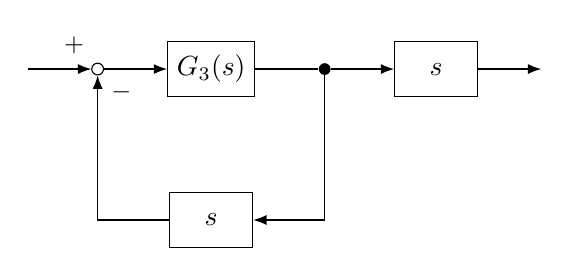
\begin{tikzpicture}[auto, node distance=0.8cm and 0.8cm, >=Latex]

      % --- 上段ノード ---
      \node[input] (input) {};
      \node[circle, draw, inner sep=1.5pt, right=of input] (sum) {};            % 合流点
      \node[block, right=of sum] (G3) {$G_3(s)$};                               % G_3(s)
      \node[circle, fill=black, inner sep=1.5pt, right=of G3] (branch) {};      % 分岐点
      \node[block, right=of branch] (S1) {$s$};                                 % 上の S
      \node[output, right=of S1] (output) {};
    
      % --- 下段ノード ---
      \node[block, below=1.2cm of G3] (S2) {$s$};                                % 下の S
    
      % --- 線描画 ---
      \draw[->] (input) -- (sum);
      \draw[->] (sum) -- (G3);
      \draw[-] (G3) -- (branch);
      \draw[->] (branch) -- (S1);
      \draw[->] (S1) -- (output);
    
      \draw[->] (branch) |- (S2);        % 分岐点から下のSへ
      \draw[->] (S2) -| (sum);           % 下のSから合流点へ
    
      % --- 加算記号 ---
      \node at ($(sum)+(-0.3,0.3)$) {\small $+$};
      \node at ($(sum)+(0.3,-0.3)$) {\small $-$};
    
    \end{tikzpicture}
  \end{center}
  
\end{minipage}\\

\begin{tcolorbox}[title={2. (1)
    \begin{center}
        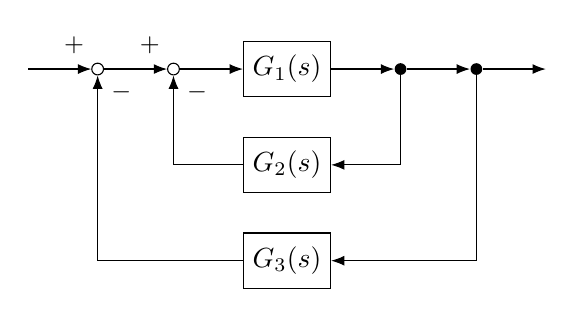
\begin{tikzpicture}[auto, node distance=0.8cm and 0.8cm, >=Latex]

        % --- 上段ノード ---
        \node[input] (input) {};
        \node[circle, draw, inner sep=1.5pt, right=of input] (sum1) {};           % 合流点①
        \node[circle, draw, inner sep=1.5pt, right=of sum1] (sum2) {}; % 合流点②
        \node[block, right=of sum2] (G1) {$G_1(s)$};              % G1
        \node[circle, fill=black, inner sep=1.5pt, right=of G1] (branch1) {}; % 分岐点①
        \node[circle, fill=black, inner sep=1.5pt, right=of branch1] (branch2) {}; % 分岐点②
        \node[output, right=of branch2] (output) {};
        
        % --- 下段ノード ---
        \node[block, below=0.5cm of G1] (G2) {$G_2(s)$};     % G2
        \node[block, below=0.5cm of G2] (G3) {$G_3(s)$};     % G3
        
        % --- 線描画 ---
        \draw[->] (input) -- (sum1);
        \draw[->] (sum1) -- (sum2);
        \draw[->] (sum2) -- (G1);
        \draw[->] (G1) -- (branch1);
        \draw[->] (branch1) -- (branch2);
        \draw[->] (branch2) -- (output);
        
        \draw[->] (branch1) |- (G2);        % 下向き:G2
        \draw[->] (G2) -| (sum2);          % 上に戻る:sum2
        
        \draw[->] (branch2) |- (G3);        % 下向き:G3
        \draw[->] (G3) -| (sum1);          % 上に戻る:sum1
        
        % --- 加算記号 ---
        \node at ($(sum1)+(-0.3,0.3)$) {\small $+$};
        \node at ($(sum1)+(0.3,-0.3)$) {\small $-$};
        \node at ($(sum2)+(-0.3,0.3)$) {\small $+$};
        \node at ($(sum2)+(0.3,-0.3)$) {\small $-$};
        
        \end{tikzpicture}
    \end{center} }]

\begin{center}
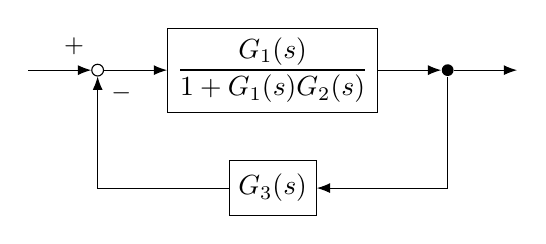
\begin{tikzpicture}[auto, node distance=0.8cm and 0.8cm, >=Latex]

  % --- 上段ノード ---
  \node[input] (input) {};
  \node[circle, draw, inner sep=1.5pt, right=of input] (sum1) {};              % 合流点①
  \node[block, right=of sum1] (G1G2) {$\dfrac{G_1(s)}{1 + G_1(s) G_2(s)}$};    % G1+G2合成済
  \node[circle, fill=black, inner sep=1.5pt, right=of G1G2] (branch2) {};      % 分岐点②
  \node[output, right=of branch2] (output) {};

  % --- 下段ノード ---
  \node[block, below=0.6cm of G1G2] (G3) {$G_3(s)$};

  % --- 線描画 ---
  \draw[->] (input) -- (sum1);
  \draw[->] (sum1) -- (G1G2);
  \draw[->] (G1G2) -- (branch2);
  \draw[->] (branch2) -- (output);

  \draw[->] (branch2) |- (G3);
  \draw[->] (G3) -| (sum1);

  % --- 加算記号 ---
  \node at ($(sum1)+(-0.3,0.3)$) {\small $+$};
  \node at ($(sum1)+(0.3,-0.3)$) {\small $-$};

\end{tikzpicture}


\vspace{2mm}
    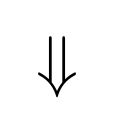
\begin{tikzpicture}
    \node {\Huge$\Downarrow$};
    \end{tikzpicture}
\vspace{2mm}


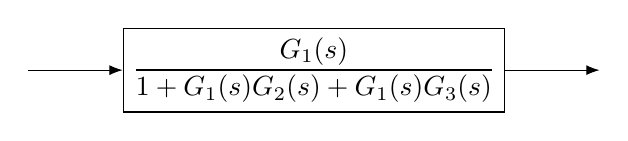
\begin{tikzpicture}[auto, node distance=1.5cm and 1.2cm, >=Latex]

  % --- ノード配置 ---
  \node[input] (input) {};
  \node[block, right=of input] (Gfinal) {$\dfrac{G_1(s)}{1 + G_1(s) G_2(s) + G_1(s) G_3(s)}$};
  \node[output, right=of Gfinal] (output) {};

  % --- 線描画 ---
  \draw[->] (input) -- (Gfinal);
  \draw[->] (Gfinal) -- (output);

\end{tikzpicture}
\end{center}

よってシステム全体の伝達関数は\\
\[
G_{all}(s)=\dfrac{G_1(s)}{1 + G_1(s) G_2(s) + G_1(s) G_3(s)}
\]


\end{tcolorbox}

\begin{tcolorbox}[title={2. (2)
    \begin{center}
    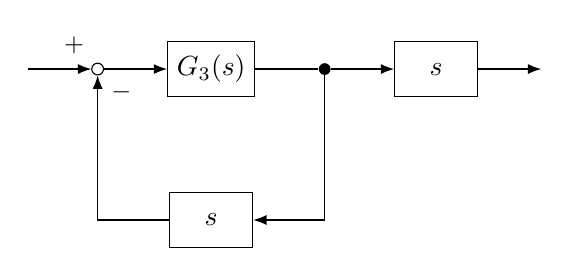
\begin{tikzpicture}[auto, node distance=0.8cm and 0.8cm, >=Latex]

        % --- 上段ノード ---
        \node[input] (input) {};
        \node[circle, draw, inner sep=1.5pt, right=of input] (sum) {};            % 合流点
        \node[block, right=of sum] (G3) {$G_3(s)$};                               % G_3(s)
        \node[circle, fill=black, inner sep=1.5pt, right=of G3] (branch) {};      % 分岐点
        \node[block, right=of branch] (S1) {$s$};                                 % 上の S
        \node[output, right=of S1] (output) {};

        % --- 下段ノード ---
        \node[block, below=1.2cm of G3] (S2) {$s$};                                % 下の S

        % --- 線描画 ---
        \draw[->] (input) -- (sum);
        \draw[->] (sum) -- (G3);
        \draw[-] (G3) -- (branch);
        \draw[->] (branch) -- (S1);
        \draw[->] (S1) -- (output);

        \draw[->] (branch) |- (S2);        % 分岐点から下のSへ
        \draw[->] (S2) -| (sum);           % 下のSから合流点へ

        % --- 加算記号 ---
        \node at ($(sum)+(-0.3,0.3)$) {\small $+$};
        \node at ($(sum)+(0.3,-0.3)$) {\small $-$};

    \end{tikzpicture}
    \end{center}}]

\begin{center}
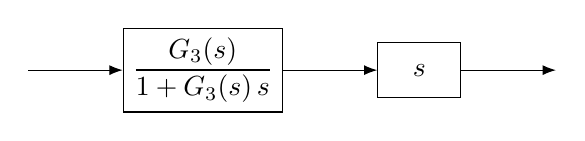
\begin{tikzpicture}[auto, node distance=0.8cm and 1.2cm, >=Latex]

  % --- ノード配置(不要ノード除去後) ---
  \node[input] (input) {};
  \node[block, right=of input] (G3fb) {$\dfrac{G_3(s)}{1 + G_3(s)\,s}$};
  \node[block, right=of G3fb] (S1) {$s$};
  \node[output, right=of S1] (output) {};

  % === 主系列 ===
  \draw[->] (input) -- (G3fb);
  \draw[->] (G3fb) -- (S1);
  \draw[->] (S1) -- (output);

\end{tikzpicture}

\vspace{2mm}
    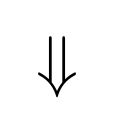
\begin{tikzpicture}
    \node {\Huge$\Downarrow$};
    \end{tikzpicture}
\vspace{2mm}


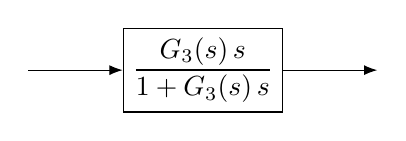
\begin{tikzpicture}[auto, node distance=1.5cm and 1.2cm, >=Latex]

  % --- ノード構成 ---
  \node[input] (input) {};
  \node[block, right=of input] (Gfinal) {$\dfrac{G_3(s)\,s}{1 + G_3(s)\,s}$};
  \node[output, right=of Gfinal] (output) {};

  % --- 線描画 ---
  \draw[->] (input) -- (Gfinal);
  \draw[->] (Gfinal) -- (output);

\end{tikzpicture}

\end{center}

よってシステム全体の伝達関数は\\
\[
G_{all}(s)=\dfrac{G_3(s)\,s}{1 + G_3(s)\,s}
\]


\end{tcolorbox}


% ---------------[3]--------------- 済
\begin{tcolorbox}[title={3. 問2.の(2)のシステムについて、\(G_3(s)=\dfrac{1}{s+3}\)のとき、単位ステップ入力を印加した際の応答を求めよ。
また、定常状態における値が存在すれば、その値を求めよ。}]

問2.の(2)より
\begin{align*}
G_{all}(s) &=  \dfrac{\frac{1}{s+3}\,s}{1 + \frac{1}{s+3}\,s} \\
            &= \dfrac{s}{2s+3}
\end{align*}
単位ステップ入力\(U(s)=\dfrac{1}{s}\)と\(Y(s)=G(S)U(S)\)より、
\begin{align*}
    &\qquad Y(s) =\frac{1}{2s+3} \\
    &\Leftrightarrow \mathcal{L}^{-1} \left[ Y(s) \right]
    =\mathcal{L}^{-1} \left[ \frac{1}{2s+3} \right]\\
    &\Leftrightarrow y(t) =  \frac{1}{2}e^{-\frac{3}{2}t}
\end{align*}
また定常値は
\[
\lim_{t \to \infty} y(t) = \lim_{t \to \infty} \frac{1}{2} e^{-\frac{3}{2}t} = 0
\]
\end{tcolorbox}

\newpage

% ---------------[4]---------------
\begin{tcolorbox}[title={4.(1) ブロック線図を簡単にせよ. 
\begin{center}
\begin{tikzpicture}[auto, node distance=0.4cm and 0.6cm, >=Latex]
  % --- 主系列ノード ---
  \node at (0,0) (input) {};
  \node[circle, draw, inner sep=1.5pt, right=of input] (sum1) {};         % 合流点1
  \node[block, right=of sum1] (G1) {$G_1$};
  \node[circle, fill=black, inner sep=1.5pt, right=of G1] (branch1) {};   % 分岐点1
  \node[block, right=of branch1] (G2) {$G_2$};
  \node[circle, fill=black, inner sep=1.5pt, right=of G2] (branch2) {};   % 分岐点2
  \node[block, right=of branch2] (G3) {$G_3$};
  \node[circle, draw, inner sep=1.5pt, right=of G3] (sum2) {};           % 合流点2
  \node[right=of sum2] (output) {};
  
  % --- 上部ノード(分岐2の上にG4) ---
  \node[block, above=0.6cm of branch2] (G4) {$G_4$};
  
  % --- 下部ノード(G1の下にH1、さらにその下にH2) ---
  \node[block, below=0.6cm of G1] (H1) {$H_1$};
  \node[block, below=0.6cm of H1] (H2) {$H_2$};

  % === 主系列経路 ===
  \draw[->] (input) -- (sum1);
  \draw[->] (sum1) -- (G1);
  \draw[->] (G1) -- (branch1);
  \draw[->] (branch1) -- (G2);
  \draw[->] (G2) -- (branch2);
  \draw[->] (branch2) -- (G3);
  \draw[->] (G3) -- (sum2);
  \draw[->] (sum2) -- (output);
  
  % === 追加経路 ===
  % 分岐1 → G4 → 合流2(カクカク経路)
  \draw[->] (branch1) |- (G4) -| (sum2);

  % 分岐1 → H1 → 合流1(カクカク経路)
  \draw[->] (branch1) |- (H1) -| (sum1);

  % 分岐2 → H2 → 合流1(カクカク経路)
  \draw[->] (branch2) |- (H2) -| (sum1);

  % --- 加算記号配置 ---
  \node at ($(sum1)+(-0.3,0.3)$) {\small $+$};
  \node at ($(sum1)+(0.3,-0.3)$) {\small $-$};
  \node at ($(sum2)+(-0.3,0.3)$) {\small $+$};
  \node at ($(sum2)+(-0.3,-0.3)$) {\small $+$};

  % --- ラベル ---
  \node at ($(sum1)+(-1.0,0.3)$) {\small $R(s)$};
  \node at ($(sum2)+(1.0,0.3)$) {\small $C(s)$};

\end{tikzpicture}
\end{center}

\vspace{2mm}
}]

\begin{center}

\begin{tikzpicture}[auto, node distance=0.4cm and 0.6cm, >=Latex]
  % --- 主系列ノード(G2とbranch2を交換) ---
  \node at (0,0) (input) {};
  \node[circle, draw, inner sep=1.5pt, right=of input] (sum1) {};         
  \node[block, right=of sum1] (G1) {$G_1$};
  \node[circle, fill=black, inner sep=1.5pt, right=of G1] (branch1) {};   
  \node[circle, fill=black, inner sep=1.5pt, right=1.2cm of branch1] (branch2) {}; % ← G2と交換された分岐点
  \node[block, right=of branch2] (G2_main) {$G_2$};                         % ← G2が後ろに
  \node[block, right=of G2_main] (G3) {$G_3$};
  \node[circle, draw, inner sep=1.5pt, right=of G3] (sum2) {};             
  \node[right=of sum2] (output) {};

  % --- 上部ノード(branch2の上にG4) ---
  \node[block, above=0.6cm of branch2] (G4) {$G_4$};

  % --- 下部ノード(G1の下にH1、G2→H2構成) ---
  \node[block, below=0.6cm of G1] (H1) {$H_1$};
  \node[block, below=0.6cm of H1] (H2) {$H_2$};
  \node[block, right=0.4cm of H2] (G2_fb) {$G_2$};  % ← G₂(H₂ルート用)
  

  % === 主系列経路 ===
  \draw[->] (input) -- (sum1);
  \draw[->] (sum1) -- (G1);
  \draw[->] (G1) -- (branch1);
  \draw[->] (branch1) -- (branch2);           % ← 分岐点2を前に
  \draw[->] (branch2) -- (G2_main);
  \draw[->] (G2_main) -- (G3);
  \draw[->] (G3) -- (sum2);
  \draw[->] (sum2) -- (output);

  % === 追加経路 ===
  \draw[->] (branch1) |- (H1) -| (sum1);
  \draw[->] (branch1) |- (G4) -| (sum2);
  \draw[->] (branch2) |- (G2_fb) -- (H2) -| (sum1);  % ← 正しく G₂ → H₂ → 合流1

  % --- 加算記号配置 ---
  \node at ($(sum1)+(-0.3,0.3)$) {\small $+$};
  \node at ($(sum1)+(0.3,-0.3)$) {\small $-$};
  \node at ($(sum2)+(-0.3,0.3)$) {\small $+$};
  \node at ($(sum2)+(-0.3,-0.3)$) {\small $+$};

  % --- ラベル ---
  \node at ($(sum1)+(-1.0,0.3)$) {\small $R(s)$};
  \node at ($(sum2)+(1.0,0.3)$) {\small $C(s)$};

\end{tikzpicture}


\vspace{2mm}
    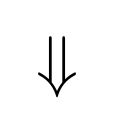
\begin{tikzpicture}
    \node {\Huge$\Downarrow$};
    \end{tikzpicture}
\vspace{2mm}


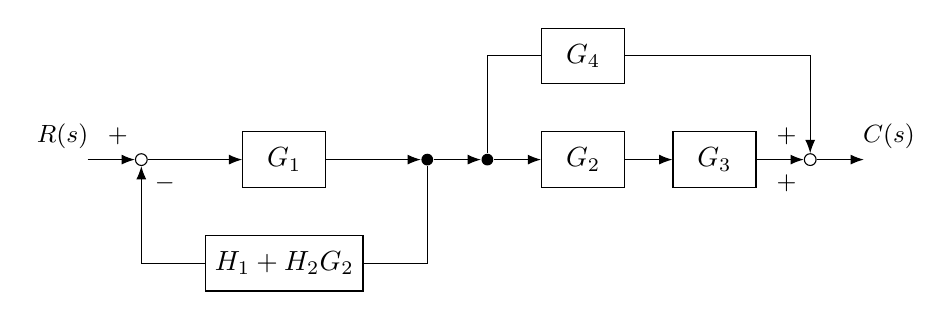
\begin{tikzpicture}[auto, node distance=0.4cm and 0.6cm, >=Latex]
  % --- 主系列ノード ---
  \node at (0,0) (input) {};
  \node[circle, draw, inner sep=1.5pt, right=of input] (sum1) {};         
  \node[block, right=1.2cm of sum1] (G1) {$G_1$};
  \node[circle, fill=black, inner sep=1.5pt, right=1.2cm of G1] (branch1) {};   
  \node[circle, fill=black, inner sep=1.5pt, right=of branch1] (branch3) {}; % ← 旧branch2削除済
  \node[block, right=of branch3] (G2_main) {$G_2$};
  \node[block, right=of G2_main] (G3) {$G_3$};
  \node[circle, draw, inner sep=1.5pt, right=of G3] (sum2) {};             
  \node[right=of sum2] (output) {};

  % --- 上部ノード(G2_mainの上にG4) ---
  \node[block, above=0.6cm of G2_main] (G4) {$G_4$};

  % --- 合成フィードバックノード(G1の真下) ---
  \node[block, below=0.6cm of G1] (Hfb) {$H_1 + H_2 G_2$};

  % === 主系列経路 ===
  \draw[->] (input) -- (sum1);
  \draw[->] (sum1) -- (G1);
  \draw[->] (G1) -- (branch1);
  \draw[->] (branch1) -- (branch3);
  \draw[->] (branch3) -- (G2_main);
  \draw[->] (G2_main) -- (G3);
  \draw[->] (G3) -- (sum2);
  \draw[->] (sum2) -- (output);

  % === 追加経路 ===
  \draw[->] (branch3) |- (G4) -| (sum2);           % 分岐3 → G4 → 合流点2
  \draw[->] (branch1) |- (Hfb) -| (sum1);          % 合成フィードバック → 合流点1

  % --- 加算記号配置 ---
  \node at ($(sum1)+(-0.3,0.3)$) {\small $+$};
  \node at ($(sum1)+(0.3,-0.3)$) {\small $-$};
  \node at ($(sum2)+(-0.3,0.3)$) {\small $+$};
  \node at ($(sum2)+(-0.3,-0.3)$) {\small $+$};

  % --- ラベル ---
  \node at ($(sum1)+(-1.0,0.3)$) {\small $R(s)$};
  \node at ($(sum2)+(1.0,0.3)$) {\small $C(s)$};

\end{tikzpicture}


\vspace{2mm}
    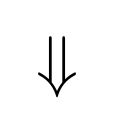
\begin{tikzpicture}
    \node {\Huge$\Downarrow$};
    \end{tikzpicture}
\vspace{2mm}


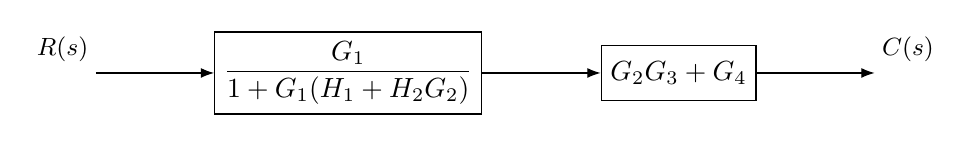
\begin{tikzpicture}[auto, node distance=1.0cm and 1.5cm, >=Latex]
  % --- 入出力とブロック ---
  \node at (0,0) (input) {};
  \node[block, right=of input] (Gleft) {$\dfrac{G_1}{1 + G_1 (H_1 + H_2 G_2)}$};
  \node[block, right=of Gleft] (Gright) {$G_2 G_3 + G_4$};
  \node[right=of Gright] (output) {};

  % --- 矢印 ---
  \draw[->] (input) -- (Gleft);
  \draw[->] (Gleft) -- (Gright);
  \draw[->] (Gright) -- (output);

  % --- ラベル ---
  \node at ($(input)+(-0.3,0.3)$) {\small $R(s)$};
  \node at ($(output)+(0.3,0.3)$) {\small $C(s)$};
\end{tikzpicture}


\vspace{2mm}
    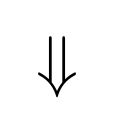
\begin{tikzpicture}
    \node {\Huge$\Downarrow$};
    \end{tikzpicture}
\vspace{2mm}


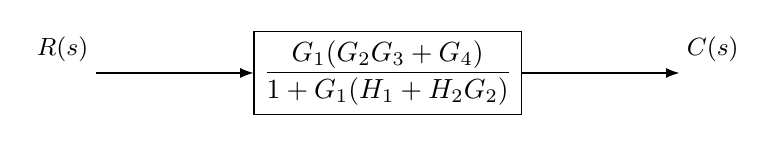
\begin{tikzpicture}[auto, node distance=1.2cm and 2.0cm, >=Latex]
  % --- 入出力とブロック ---
  \node at (0,0) (input) {};
  \node[block, right=of input] (Gtotal) 
    {$\dfrac{G_1 (G_2 G_3 + G_4)}{1 + G_1 (H_1 + H_2 G_2)}$};
  \node[right=of Gtotal] (output) {};

  % --- 矢印 ---
  \draw[->] (input) -- (Gtotal);
  \draw[->] (Gtotal) -- (output);

  % --- ラベル ---
  \node at ($(input)+(-0.3,0.3)$) {\small $R(s)$};
  \node at ($(output)+(0.3,0.3)$) {\small $C(s)$};
\end{tikzpicture}

\end{center}

\end{tcolorbox}

\begin{tcolorbox}[title={4.(2) ブロック線図を簡単にせよ. 
\begin{center}
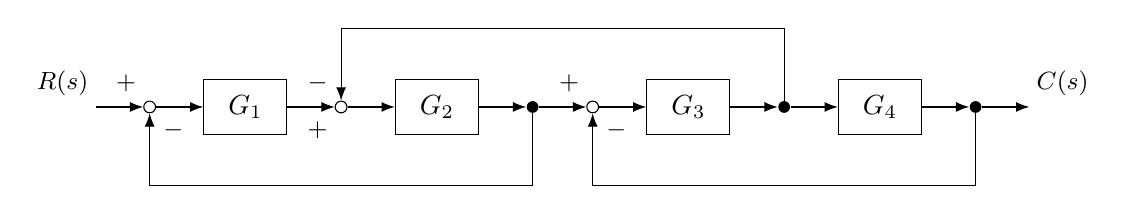
\begin{tikzpicture}[auto, node distance=0.4cm and 0.6cm, >=Latex]

  % --- 主系列ノード配置 ---
  \node at (0,0) (input) {};
  \node[circle, draw, inner sep=1.5pt, right=of input] (sum1) {};          % 合流1
  \node[block, right=of sum1] (G1) {$G_1$};
  \node[circle, draw, inner sep=1.5pt, right=of G1] (sum2) {};             % 合流2
  \node[block, right=of sum2] (G2) {$G_2$};
  \node[circle, fill=black, inner sep=1.5pt, right=of G2] (branch1) {};    % 分岐1
  \node[circle, draw, inner sep=1.5pt, right=of branch1] (sum3) {};        % 合流3
  \node[block, right=of sum3] (G3) {$G_3$};
  \node[circle, fill=black, inner sep=1.5pt, right=of G3] (branch2) {};    % 分岐2
  \node[block, right=of branch2] (G4) {$G_4$};
  \node[circle, fill=black, inner sep=1.5pt, right=of G4] (branch3) {};    % 分岐3
  \node[right=of branch3] (output) {};

  % --- 経由ポイント(カクカク折れ線用) ---
  \coordinate (pivot1) at ($(branch1)+(0,-1.0)$);  % branch1 → sum1
  \coordinate (pivot2) at ($(branch2)+(0,1.0)$);   % branch2 → sum2
  \coordinate (pivot3) at ($(branch3)+(0,-1.0)$);  % branch3 → sum3

  % === 主系列経路 ===
  \draw[->] (input) -- (sum1);
  \draw[->] (sum1) -- (G1);
  \draw[->] (G1) -- (sum2);
  \draw[->] (sum2) -- (G2);
  \draw[->] (G2) -- (branch1);
  \draw[->] (branch1) -- (sum3);
  \draw[->] (sum3) -- (G3);
  \draw[->] (G3) -- (branch2);
  \draw[->] (branch2) -- (G4);
  \draw[->] (G4) -- (branch3);
  \draw[->] (branch3) -- (output);

  % === 追加経路(折れ線) ===
  \draw[->] (branch1) -- (pivot1) -| (sum1);
  \draw[->] (branch2) -- (pivot2) -| (sum2);
  \draw[->] (branch3) -- (pivot3) -| (sum3);

  % --- 加算記号配置 ---
  \node at ($(sum1)+(-0.3,0.3)$) {\small $+$};
  \node at ($(sum1)+(0.3,-0.3)$) {\small $-$};

  \node at ($(sum2)+(-0.3,0.3)$) {\small $-$};
  \node at ($(sum2)+(-0.3,-0.3)$) {\small $+$};

  \node at ($(sum3)+(-0.3,0.3)$) {\small $+$};
  \node at ($(sum3)+(0.3,-0.3)$) {\small $-$};

  % --- 入出力ラベル ---
  \node at ($(input)+(-0.3,0.3)$) {\small $R(s)$};
  \node at ($(output)+(0.3,0.3)$) {\small $C(s)$};

\end{tikzpicture}
\end{center}

\vspace{2mm}
}]

\begin{center}

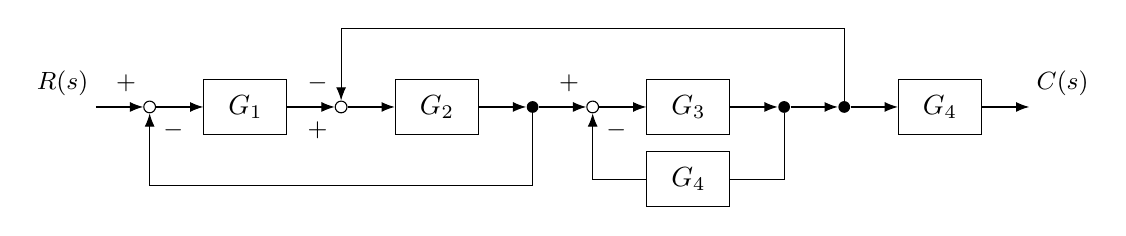
\begin{tikzpicture}[auto, node distance=0.4cm and 0.6cm, >=Latex]

  % --- 主系列ノード配置 ---
  \node at (0,0) (input) {};
  \node[circle, draw, inner sep=1.5pt, right=of input] (sum1) {};         
  \node[block, right=of sum1] (G1) {$G_1$};
  \node[circle, draw, inner sep=1.5pt, right=of G1] (sum2) {};            
  \node[block, right=of sum2] (G2) {$G_2$};
  \node[circle, fill=black, inner sep=1.5pt, right=of G2] (branch1) {};   
  \node[circle, draw, inner sep=1.5pt, right=of branch1] (sum3) {};       
  \node[block, right=of sum3] (G3) {$G_3$};
  \node[circle, fill=black, inner sep=1.5pt, right=of G3] (branch3) {};   % 分岐3:G3と分岐2の間
  \node[circle, fill=black, inner sep=1.5pt, right=of branch3] (branch2) {}; 
  \node[block, right=of branch2] (G4_main) {$G_4$};                       % 主系列上のG4
  \node[right=of G4_main] (output) {};

  % --- G4(追加ルート用) ---
  \node[block, below=0.2cm of G3] (G4_fb) {$G_4$}; % G3の下

  % --- 経由ポイント ---
  \coordinate (pivot1) at ($(branch1)+(0,-1.0)$);  % branch1 → sum1
  \coordinate (pivot2) at ($(branch2)+(0,1.0)$);   % branch2 → sum2

  % === 主系列経路 ===
  \draw[->] (input) -- (sum1);
  \draw[->] (sum1) -- (G1);
  \draw[->] (G1) -- (sum2);
  \draw[->] (sum2) -- (G2);
  \draw[->] (G2) -- (branch1);
  \draw[->] (branch1) -- (sum3);
  \draw[->] (sum3) -- (G3);
  \draw[->] (G3) -- (branch3);
  \draw[->] (branch3) -- (branch2);
  \draw[->] (branch2) -- (G4_main);
  \draw[->] (G4_main) -- (output);

  % === 追加経路 ===
  \draw[->] (branch1) -- (pivot1) -| (sum1);
  \draw[->] (branch2) -- (pivot2) -| (sum2);
  \draw[->] (branch3) |- (G4_fb) -| (sum3);  % ← G4経由の戻りルート

  % --- 加算記号配置 ---
  \node at ($(sum1)+(-0.3,0.3)$) {\small $+$};
  \node at ($(sum1)+(0.3,-0.3)$) {\small $-$};

  \node at ($(sum2)+(-0.3,0.3)$) {\small $-$};
  \node at ($(sum2)+(-0.3,-0.3)$) {\small $+$};

  \node at ($(sum3)+(-0.3,0.3)$) {\small $+$};
  \node at ($(sum3)+(0.3,-0.3)$) {\small $-$};

  % --- ラベル ---
  \node at ($(input)+(-0.3,0.3)$) {\small $R(s)$};
  \node at ($(output)+(0.3,0.3)$) {\small $C(s)$};

\end{tikzpicture}


\vspace{2mm}
    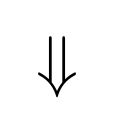
\begin{tikzpicture}
    \node {\Huge$\Downarrow$};
    \end{tikzpicture}
\vspace{2mm}

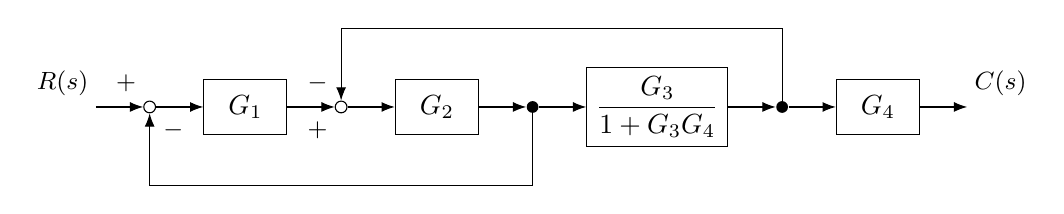
\begin{tikzpicture}[auto, node distance=0.4cm and 0.6cm, >=Latex]

  % --- 主系列ノード配置 ---
  \node at (0,0) (input) {};
  \node[circle, draw, inner sep=1.5pt, right=of input] (sum1) {};         
  \node[block, right=of sum1] (G1) {$G_1$};
  \node[circle, draw, inner sep=1.5pt, right=of G1] (sum2) {};            
  \node[block, right=of sum2] (G2) {$G_2$};
  \node[circle, fill=black, inner sep=1.5pt, right=of G2] (branch1) {};   
  \node[block, right=of branch1] (G3_fb) {$\dfrac{G_3}{1 + G_3 G_4}$};     % フィードバック済
  \node[circle, fill=black, inner sep=1.5pt, right=of G3_fb] (branch2) {}; 
  \node[block, right=of branch2] (G4_main) {$G_4$};
  \node[right=of G4_main] (output) {};

  % --- 経由ポイント ---
  \coordinate (pivot1) at ($(branch1)+(0,-1.0)$);  % branch1 → sum1
  \coordinate (pivot2) at ($(branch2)+(0,1.0)$);   % branch2 → sum2

  % === 主系列経路 ===
  \draw[->] (input) -- (sum1);
  \draw[->] (sum1) -- (G1);
  \draw[->] (G1) -- (sum2);
  \draw[->] (sum2) -- (G2);
  \draw[->] (G2) -- (branch1);
  \draw[->] (branch1) -- (G3_fb);
  \draw[->] (G3_fb) -- (branch2);
  \draw[->] (branch2) -- (G4_main);
  \draw[->] (G4_main) -- (output);

  % === 追加経路 ===
  \draw[->] (branch1) -- (pivot1) -| (sum1);
  \draw[->] (branch2) -- (pivot2) -| (sum2);

  % --- 加算記号配置 ---
  \node at ($(sum1)+(-0.3,0.3)$) {\small $+$};
  \node at ($(sum1)+(0.3,-0.3)$) {\small $-$};

  \node at ($(sum2)+(-0.3,0.3)$) {\small $-$};
  \node at ($(sum2)+(-0.3,-0.3)$) {\small $+$};

  % --- ラベル ---
  \node at ($(input)+(-0.3,0.3)$) {\small $R(s)$};
  \node at ($(output)+(0.3,0.3)$) {\small $C(s)$};

\end{tikzpicture}



\vspace{2mm}
    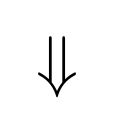
\begin{tikzpicture}
    \node {\Huge$\Downarrow$};
    \end{tikzpicture}
\vspace{2mm}

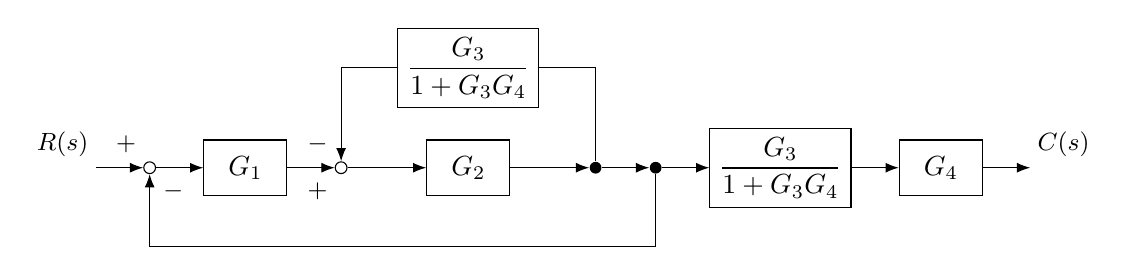
\begin{tikzpicture}[auto, node distance=0.4cm and 0.6cm, >=Latex]

  % --- 主系列ノード配置 ---
  \node at (0,0) (input) {};
  \node[circle, draw, inner sep=1.5pt, right=of input] (sum1) {};         
  \node[block, right=of sum1] (G1) {$G_1$};
  \node[circle, draw, inner sep=1.5pt, right=of G1] (sum2) {};            
  \node[block, right=1.0cm of sum2] (G2) {$G_2$};
  \node[circle, fill=black, inner sep=1.5pt, right=1.0cm of G2] (branch2) {};   % ← 分岐2
  \node[circle, fill=black, inner sep=1.5pt, right=of branch2] (branch1) {};   
  \node[block, right=of branch1] (G3_fb) {$\dfrac{G_3}{1 + G_3 G_4}$};     % フィードバック済
  \node[block, above=0.4cm of G2] (G3_fb_dup) {$\dfrac{G_3}{1 + G_3 G_4}$}; % 分岐2→sum2用
  \node[block, right=of G3_fb] (G4_main) {$G_4$};
  \node[right=of G4_main] (output) {};

  % --- 経由ポイント(1のみ残す) ---
  \coordinate (pivot1) at ($(branch1)+(0,-1.0)$);  % branch1 → sum1

  % === 主系列経路 ===
  \draw[->] (input) -- (sum1);
  \draw[->] (sum1) -- (G1);
  \draw[->] (G1) -- (sum2);
  \draw[->] (sum2) -- (G2);
  \draw[->] (G2) -- (branch2);
  \draw[->] (branch2) -- (branch1);
  \draw[->] (branch1) -- (G3_fb);
  \draw[->] (G3_fb) -- (G4_main);
  \draw[->] (G4_main) -- (output);

  % === 追加経路 ===
  \draw[->] (branch1) -- (pivot1) -| (sum1);
  \draw[->] (branch2) |- (G3_fb_dup) -| (sum2);   % ← pivot2 削除、直接 |- 接続

  % --- 加算記号配置 ---
  \node at ($(sum1)+(-0.3,0.3)$) {\small $+$};
  \node at ($(sum1)+(0.3,-0.3)$) {\small $-$};

  \node at ($(sum2)+(-0.3,0.3)$) {\small $-$};
  \node at ($(sum2)+(-0.3,-0.3)$) {\small $+$};

  % --- ラベル ---
  \node at ($(input)+(-0.3,0.3)$) {\small $R(s)$};
  \node at ($(output)+(0.3,0.3)$) {\small $C(s)$};

\end{tikzpicture}


\vspace{2mm}
    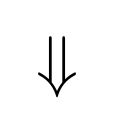
\begin{tikzpicture}
    \node {\Huge$\Downarrow$};
    \end{tikzpicture}
\vspace{2mm}

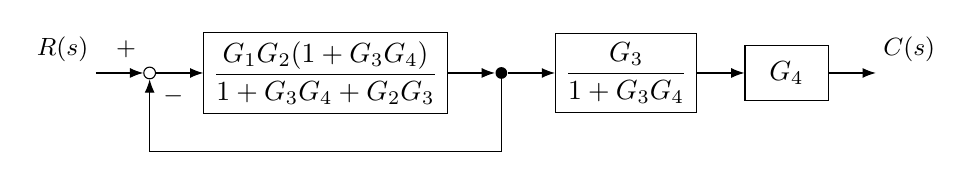
\begin{tikzpicture}[auto, node distance=0.4cm and 0.6cm, >=Latex]

  % 主系列ノード配置
  \node at (0,0) (input) {};
  \node[circle, draw, inner sep=1.5pt, right=of input] (sum1) {};
  \node[block, right=of sum1] (G1G2fb) 
    {$\dfrac{G_1 G_2 (1 + G_3 G_4)}{1 + G_3 G_4 + G_2 G_3}$}; % ← G1をかけた形
  \node[circle, fill=black, inner sep=1.5pt, right=of G1G2fb] (branch1) {};
  \node[block, right=of branch1] (G3_fb) {$\dfrac{G_3}{1 + G_3 G_4}$};
  \node[block, right=of G3_fb] (G4_main) {$G_4$};
  \node[right=of G4_main] (output) {};

  % 経由ポイント(sum1フィードバック用)
  \coordinate (pivot1) at ($(branch1)+(0,-1.0)$);

  % 主系列経路
  \draw[->] (input) -- (sum1);
  \draw[->] (sum1) -- (G1G2fb);
  \draw[->] (G1G2fb) -- (branch1);
  \draw[->] (branch1) -- (G3_fb);
  \draw[->] (G3_fb) -- (G4_main);
  \draw[->] (G4_main) -- (output);

  % フィードバック経路
  \draw[->] (branch1) -- (pivot1) -| (sum1);

  % 加算記号
  \node at ($(sum1)+(-0.3,0.3)$) {\small $+$};
  \node at ($(sum1)+(0.3,-0.3)$) {\small $-$};

  % ラベル
  \node at ($(input)+(-0.3,0.3)$) {\small $R(s)$};
  \node at ($(output)+(0.3,0.3)$) {\small $C(s)$};

\end{tikzpicture}



\vspace{2mm}
    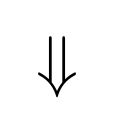
\begin{tikzpicture}
    \node {\Huge$\Downarrow$};
    \end{tikzpicture}
\vspace{2mm}

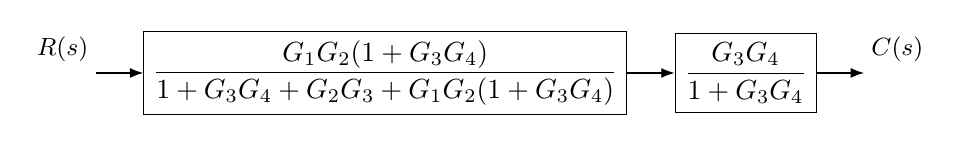
\begin{tikzpicture}[auto, node distance=0.4cm and 0.6cm, >=Latex]

  % ノード配置
  \node at (0,0) (input) {};
  \node[block, right=of input] (Gleft) 
    {$\dfrac{G_1 G_2 (1 + G_3 G_4)}{1 + G_3 G_4 + G_2 G_3 + G_1 G_2 (1 + G_3 G_4)}$};
  \node[block, right=of Gleft] (Gright) 
    {$\dfrac{G_3 G_4}{1 + G_3 G_4}$};
  \node[right=of Gright] (output) {};

  % 矢印
  \draw[->] (input) -- (Gleft);
  \draw[->] (Gleft) -- (Gright);
  \draw[->] (Gright) -- (output);

  % ラベル
  \node at ($(input)+(-0.3,0.3)$) {\small $R(s)$};
  \node at ($(output)+(0.3,0.3)$) {\small $C(s)$};

\end{tikzpicture}


\vspace{2mm}
    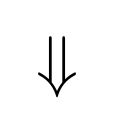
\begin{tikzpicture}
    \node {\Huge$\Downarrow$};
    \end{tikzpicture}
\vspace{2mm}

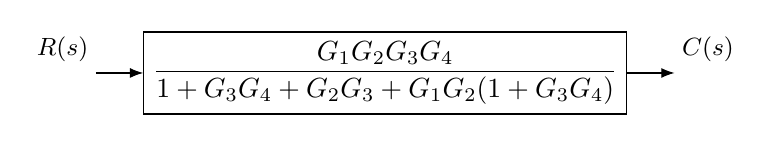
\begin{tikzpicture}[auto, node distance=0.4cm and 0.6cm, >=Latex]

  % ノード配置
  \node at (0,0) (input) {};
  \node[block, right=of input] (Gfinal) 
    {
    $\dfrac{
      G_1 G_2 G_3 G_4
    }{
      1 + G_3 G_4 + G_2 G_3 + G_1 G_2 (1 + G_3 G_4)
    }$
    };
  \node[right=of Gfinal] (output) {};

  % 矢印
  \draw[->] (input) -- (Gfinal);
  \draw[->] (Gfinal) -- (output);

  % ラベル
  \node at ($(input)+(-0.3,0.3)$) {\small $R(s)$};
  \node at ($(output)+(0.3,0.3)$) {\small $C(s)$};

\end{tikzpicture}


\end{center}

\end{tcolorbox}

% ---------------[5]---------------
\begin{tcolorbox}[title={5.下図に示すフィードバックシステムにおいて、\(G_1(s)=\dfrac{1}{s+2},G_2(s)=s,G_3(s)=K_1\)
となるとき、ステップ応答における定常値が1になるよう、\(K_1\)を定めよ。\\
\begin{center}
  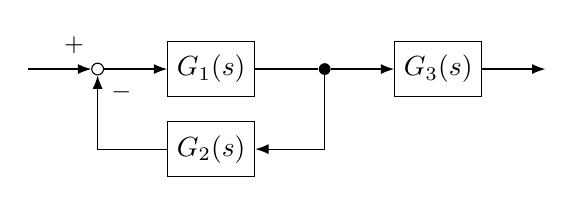
\begin{tikzpicture}[auto, node distance=0.8cm and 0.8cm, >=Latex]

    % --- 上段ノード ---
    \node[input] (input) {};
    \node[circle, draw, inner sep=1.5pt, right=of input] (sum) {};            % 合流点
    \node[block, right=of sum] (G3) {$G_1(s)$};                               % G_3(s)
    \node[circle, fill=black, inner sep=1.5pt, right=of G3] (branch) {};      % 分岐点
    \node[block, right=of branch] (S1) {$G_3(s)$};                                 % 上の S
    \node[output, right=of S1] (output) {};
  
    % --- 下段ノード ---
    \node[block, below=0.3cm of G3] (S2) {$G_2(s)$};                                % 下の S
  
    % --- 線描画 ---
    \draw[->] (input) -- (sum);
    \draw[->] (sum) -- (G3);
    \draw[-] (G3) -- (branch);
    \draw[->] (branch) -- (S1);
    \draw[->] (S1) -- (output);
  
    \draw[->] (branch) |- (S2);        % 分岐点から下のSへ
    \draw[->] (S2) -| (sum);           % 下のSから合流点へ
  
    % --- 加算記号 ---
    \node at ($(sum)+(-0.3,0.3)$) {\small $+$};
    \node at ($(sum)+(0.3,-0.3)$) {\small $-$};
  
  \end{tikzpicture}
\end{center}}]
\begin{center}
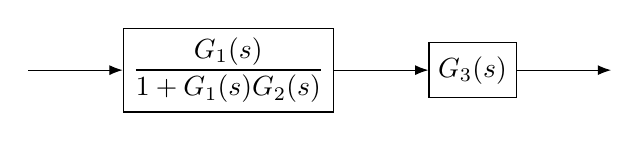
\begin{tikzpicture}[auto, node distance=0.8cm and 1.2cm, >=Latex]

  % --- ノード構成 ---
  \node[input] (input) {};
  \node[block, right=of input] (G1G2) {$\dfrac{G_1(s)}{1 + G_1(s) G_2(s)}$};
  \node[block, right=of G1G2] (G3) {$G_3(s)$};
  \node[output, right=of G3] (output) {};

  % --- 線描画 ---
  \draw[->] (input) -- (G1G2);
  \draw[->] (G1G2) -- (G3);
  \draw[->] (G3) -- (output);

\end{tikzpicture}

\vspace{2mm}
    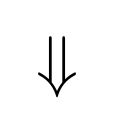
\begin{tikzpicture}
    \node {\Huge$\Downarrow$};
    \end{tikzpicture}
\vspace{2mm}

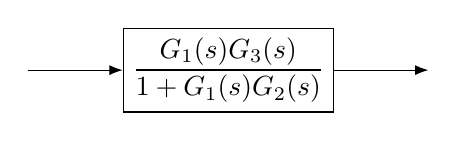
\begin{tikzpicture}[auto, node distance=1.5cm and 1.2cm, >=Latex]

  % --- ノード構成 ---
  \node[input] (input) {};
  \node[block, right=of input] (Gfinal) {$\dfrac{G_1(s) G_3(s)}{1 + G_1(s) G_2(s)}$};
  \node[output, right=of Gfinal] (output) {};

  % --- 線描画 ---
  \draw[->] (input) -- (Gfinal);
  \draw[->] (Gfinal) -- (output);

\end{tikzpicture}
\end{center}
\vspace{-4mm}
よってシステム全体の伝達関数は
\vspace{-4mm}
\begin{align*}
  G_{all}(s) &=\dfrac{G_1(s) G_3(s)}{1 + G_1(s) G_2(s)} \\
            & =\dfrac{\frac{1}{s+2} K_1}{1 +\frac{1}{s+2} \cdot s} \\
            & =\dfrac{K_1}{2(s+1)}
\end{align*}
単位ステップ入力\(U(s)=\frac{1}{s}\)とすると、単位ステップ応答\(X(s)\)は
\vspace{-3mm}
\begin{align*}
    &\qquad X(s) =G_{all}(s) U(s)=\dfrac{K_1}{2s(s+1)} \\
    &\Leftrightarrow X(s) = \frac{K_1}{2}\left(\frac{1}{s} - \frac{1}{s+1} \right) \\
    &\Leftrightarrow \mathcal{L}^{-1} \left[ X(s)  \right]
    =\mathcal{L}^{-1} \left[ \frac{K_1}{2}\left(\frac{1}{s} - \frac{1}{s+1} \right) \right]\\
    &\Leftrightarrow x(t) =  \frac{K_1}{2} \left(1-e^{-t} \right)
\end{align*}
また定常値は
\[
\lim_{t \to \infty} x(t) = \lim_{t \to \infty} \frac{K_1}{2} \left(1-e^{-t} \right) = \frac{K_1}{2}
\]
よって定常値が1になるような\(K_1\)は
\vspace{-3mm}
\[
K_1=2
\]
  \begin{tcolorbox}[title={}]
  ※最終値定理より以下のように解く方が速い
  \[
  \lim_{t \to \infty} x(t) = \lim_{s \to 0} sX(s) = \frac{K_1}{2} \therefore K_1=2
  \]
  \end{tcolorbox}
\end{tcolorbox}

\newpage

% ---------------[6]---------------
\noindent
\begin{minipage}[t]{0.005\linewidth}
    6.
\end{minipage}
\hfill
\begin{minipage}[t]{0.595\linewidth}
右図に示す系について、入力を変位\(x_1(t)\)、出力を変位\(x_2(t)\)としたとき、
次の問いに答えよ。なお、\(m\)は質量[kg]、\(d\)は粘性係数[Ns/m]、
\(k_1\)、\(k_2\)はバネ[N/m] 
とし、初期状態において系は静止しているとする。  
\end{minipage}
\hfill
\begin{minipage}[t]{0.35\linewidth}
    \vspace{-6mm}
    \begin{center}
        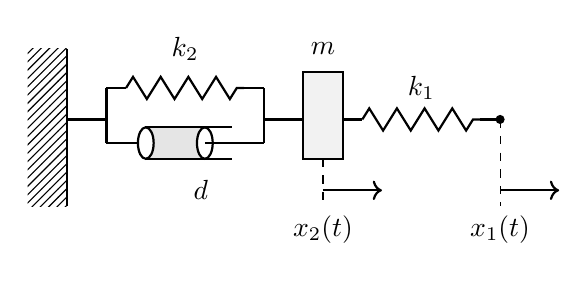
\begin{tikzpicture}[scale=1.0]
          % 固定壁
          \fill[pattern=north east lines] (-1,0,0) rectangle (-0.5,2);
          \draw[thick] (-0.5,0) -- (-0.5,2);
      
          %接続部1
          \draw[thick] (-0.5,1.1) -- (0,1.1);
          \draw[thick] (0,0.8) -- (0,1.5);
        
          % バネ2
          \draw[thick] (0,1.5) -- (0.25,1.5);
          \draw[thick, decorate, decoration={zigzag, segment length=10, amplitude=4}] (0.25,1.5) -- (1.75,1.5);
          \draw[thick] (1.75,1.5) -- (2.0,1.5);
          \node at (1.0,2.0) {$k_2$};
        
          % ダンパー(シリンダー形式)
          \draw[thick] (0,0.8) -- (0.5,0.8); % 棒
          \draw[thick, fill=gray!20] (0.5,0.6) rectangle (1.25,1.0); % 筒の側面
          \draw[thick] (1.25,1.0) -- (1.60,1.0); % 筒の上
          \draw[thick] (1.25,0.6) -- (1.60,0.6); % 筒の下
          \draw[thick, fill=white] (0.5,0.8) ellipse (0.1 and 0.2); % 左端面
          \draw[thick, fill=white] (1.25,0.8) ellipse (0.1 and 0.2); % 右端面
          \draw[thick] (1.25,0.8) -- (2.0,0.8); % ピストン棒
          \node at (1.2,0.2) {$d$};
      
          %接続部2
          \draw[thick] (2.0,0.8) -- (2.0,1.5);
          \draw[thick] (2.0,1.1) -- (2.5,1.1);
        
          % 質量M
          \draw[thick, fill=gray!10] (2.5,0.6) rectangle (3.0,1.7);
          \node at (2.75,2.0) {$m$};
      
          % バネ1
          \draw[thick] (3.0,1.1) -- (3.25,1.1);
          \draw[thick, decorate, decoration={zigzag, segment length=10, amplitude=4}] (3.25,1.1) -- (4.75,1.1);
          \draw[thick] (4.75,1.1) -- (5.0,1.1);
          \node at (4.0,1.5) {$k_1$};
      
          % 丸
          \draw[fill] (5,1.1) circle (0.05);
      
        
          % 座標x1
          \draw[->, thick] (5,0.2) -- (5.75,0.2);
          \node at (5,-0.3) {$x_1(t)$};
          \draw[dashed] (5,1.1) -- (5,0);
      
          % 座標x2
          \draw[->, thick] (2.75,0.2) -- (3.5,0.2);
          \node at (2.75,-0.3) {$x_2(t)$};
          \draw[dashed] (2.75,0.6) -- (2.75,0);
        
        \end{tikzpicture}
    \end{center}
\end{minipage}\\

\indent
(1)この図によって示されるシステムの運動方程式と伝達関数を求めよ。\\

\indent
(2)\(m=1,d=4,k_1=1,k_2=2\)とし、インパルス応答、ステップ応答をそれぞれ求\\
\indent \quad めよ。\\

\indent
(3)\(m=1,d=2,k_1=3,k_2=2\)とし、ステップ応答を求めよ。\\

\indent
(4)\(m=1,d=2,k_1=1,k_2=0\)とし、ステップ応答を求めよ。\\

\indent
(5)\(m=1,d=0,k_1=1,k_2=2\)とし、ステップ応答を求めよ。\\

\indent
(6)\(m=1,d=0,k_1=2,k_2=1\)とし、入力変位\(x_1(t)=\sin(t)\)を与えたときの応答を求
\indent \quad めよ。\\

\indent
(7)\(m=1,d=2,k_1=1,k_2=1\)とし、入力変位\(x_1(t)=\sin(2t)\)を与えたときの応答を
\indent \quad 求めよ。\\

% ---------------[6(1)]--------------- 済
\begin{tcolorbox}[title={6. (1)この図によって示されるシステムの運動方程式と伝達関数を求めよ。 
    }]

    \(x(t)\)に関する運動方程式は
    \begin{align*}
        &\qquad m\ddot{x}_2 =-k_2 x_2 - d \dot{x}_2 - k_1 \left(x_2 - x_1\right) \\
    \end{align*}
    また伝達関数は
    \begin{align*}
        &\qquad m\ddot{x}_2 +  d \dot{x}_2 + \left(k_1+k_2\right) x_2
        = k_1 x_1 \\
        &\therefore \quad \mathcal{L} \left[ m\ddot{x}_2 +  d \dot{x}_2 + \left(k_1+k_2\right) x_2\right] 
        =\mathcal{L} \left[ k_1 x_1 \right] \\
        &\therefore \quad \left\{m s^2 + d s + \left(k_1+k_2\right) \right\}\,X_2(s) = k_1 X_1(s) \quad [\because \dot{x}(0)=x(0)=0 ]\\
        &\therefore \quad G(s) \;=\;\frac{X_2(s)}{X_1(s)}
        \;=\;\frac{k_1}{m s^2 + d s + \left(k_1 + k_2\right)}
    \end{align*}

\end{tcolorbox}

% ---------------[6(2)]--------------- 済
\begin{tcolorbox}[title={6. (2)\(m=1,d=4,k_1=1,k_2=2\)とし、インパルス応答、ステップ応答をそれぞれ\\
\indent \quad 求めよ。}]

    (\uppercase\expandafter{\romannumeral 1})インパルス応答 \\
    パラメータを代入し、インパルス入力のラプラス変換は\(F(s)=1\)なので
    \vspace{-2mm}
    \begin{align*}
        &\qquad G(s) = \frac{1}{s^2 + 4 s + 3 } \\
        &\therefore \quad X(s) = G(s) F(s) = \frac{1}{(s+1)(s+3)} \\
        &\therefore \quad X(s) = \frac{1}{2} \left( \frac{1}{s+1} + \frac{-1}{s+3} \right)\\
        &\therefore \quad \mathcal{L}^{-1} \left[ X(s)\right] 
        =\frac{1}{2} \left\{ \mathcal{L}^{-1} \left[\frac{1}{s+1}\right] 
        + \mathcal{L}^{-1} \left[\frac{-1}{s+3}\right] \right\}\\
        &\therefore \quad x(t) = \frac{1}{2}\left(e^{-t} - e^{-3t} \right)
    \end{align*}

    (\uppercase\expandafter{\romannumeral 2})ステップ応答 \\
    パラメータを代入し、ステップ入力のラプラス変換は\(F(s)=\dfrac{1}{s}\)なので
    \vspace{-2mm}
    \begin{align*}
        &\qquad G(s) = \frac{1}{s^2 + 4 s + 3 } \\
        &\therefore \quad X(s) = G(s) F(s) = \frac{1}{s(s+1)(s+3)} \\
        &\therefore \quad X(s) = \frac{\frac{1}{3}}{s} 
        + \frac{\left(-\frac{1}{2}\right)}{s+1} 
        + \frac{\left(\frac{1}{6}\right)}{s+3} \\
        &\therefore \quad \mathcal{L}^{-1} \left[ X(s)\right] 
        = \mathcal{L}^{-1} \left[\frac{\left(\frac{1}{3}\right)}{s}\right] 
        + \mathcal{L}^{-1} \left[\frac{\left(-\frac{1}{2}\right)}{s+1}\right]
        + \mathcal{L}^{-1} \left[\frac{\left(\frac{1}{6}\right)}{s+3}\right] \\
        &\therefore \quad x(t) = \frac{1}{3} - \frac{1}{2}e^{-t} +\frac{1}{6} e^{-3t}
    \end{align*}

\end{tcolorbox}

% ---------------[6(3)]--------------- 済
\begin{tcolorbox}[title={6. (3)\(m=1,d=2,k_1=3,k_2=2\)とし、ステップ応答を求めよ。 
    }]
    パラメータを代入し、ステップ入力のラプラス変換は\(F(s)=\dfrac{1}{s}\)なので
    \vspace{-4mm}
    \begin{align*}
        &\qquad G(s) = \frac{3}{s^2 + 2s + 5 } \\
        &\therefore \quad X(s) = G(s) F(s) 
        = \frac{3}{s(s^2 + 2s + 5)} \\
        &\therefore \quad X(s) = \frac{\left(\frac{3}{5}\right)}{s}
        +\frac{-\frac{3}{5}s-\frac{6}{5}}{s^2 + 2s + 5} \\
        &\therefore \quad \mathcal{L}^{-1} \left[ X(s)\right] 
        = \mathcal{L}^{-1} \left[\frac{\left(\frac{3}{5}\right)}{s}\right] 
        + \mathcal{L}^{-1} \left[\frac{-\frac{3}{5}\left\{(s+1)+\frac{1}{2}\cdot 2\right\}}{\left(s+1\right)^2+2^2} \right] \\
        &\therefore \quad x(t) = \frac{3}{5} -\frac{3}{5} e^{-t} \left\{ \cos 2t + \frac{1}{2} \sin 2t\right\}
    \end{align*}

\end{tcolorbox}

% ---------------[6(4)]--------------- 済
\begin{tcolorbox}[title={6. (4)\(m=1,d=2,k_1=1,k_2=0\)とし、ステップ応答を求めよ。 
    }]
    パラメータを代入し、ステップ入力のラプラス変換は\(F(s)=\dfrac{1}{s}\)なので
    \vspace{-4mm}
    \begin{align*}
        &\qquad G(s) = \frac{1}{s^2 + 2s + 1} \\
        &\therefore \quad X(s) = G(s) F(s) = \frac{1}{s(s+1)^2} \\
        &\therefore \quad X(s) = \frac{1}{s}+\frac{-1}{(s+1)^2}+\frac{-1}{s+1} \\
        &\therefore \quad \mathcal{L}^{-1} \left[ X(s)\right] 
        = \mathcal{L}^{-1} \left[\frac{1}{s}\right] 
        + \mathcal{L}^{-1} \left[\frac{-1}{(s+1)^2} \right]
        + \mathcal{L}^{-1} \left[\frac{-1}{s+1} \right] \\
        &\therefore \quad x(t) = 1 - e^{-t}(t+1)
    \end{align*}

\end{tcolorbox}

% ---------------[6(5)]--------------- 済
\begin{tcolorbox}[title={6. (5)\(m=1,d=0,k_1=1,k_2=2\)とし、ステップ応答を求めよ。 
    }]
    パラメータを代入し、ステップ入力のラプラス変換は\(F(s)=\dfrac{1}{s}\)なので
    \vspace{-4mm}
    \begin{align*}
        &\qquad G(s) = \frac{1}{s^2 + 3} \\
        &\therefore \quad X(s) = G(s) F(s) = \frac{1}{s(s^2+3)} \\
        &\therefore \quad X(s) = \frac{\left(\frac{1}{3}\right)}{s}
        + \frac{\left(-\frac{1}{3}s\right)}{s^2+3} \\
        &\therefore \quad \mathcal{L}^{-1} \left[ X(s)\right] 
        = \mathcal{L}^{-1} \left[\frac{\left(\frac{1}{3}\right)}{s}\right] 
        + \mathcal{L}^{-1} \left[\frac{\left(-\frac{1}{3}s\right)}{s^2+3} \right] \\
        &\therefore \quad x(t) = \frac{1}{3} - \frac{1}{3}  \cos \left( \sqrt{3} t \right)
    \end{align*}

\end{tcolorbox}


% ---------------[6(6)]--------------- 済
\begin{tcolorbox}[title={6. (6)\(m=1,d=0,k_1=2,k_2=1\)とし、入力変位\(x_1(t)=\sin(t)\)を与えたときの応
\indent \quad 答を求めよ。 }]
パラメータを代入し、\(x_1(t)=\sin(t)\)のラプラス変換は\(X_i(s)=\dfrac{1}{s^2+1}\)なので
    \vspace{-4mm}
    \begin{align*}
        &\qquad G(s) = \frac{2}{s^2 +3} \\
        &\therefore \quad X(s) = G(s) F(s) = \frac{2}{(s^2 +1)(s^2+3)} \\
        &\therefore \quad X(s) =  \frac{1}{s^2 +1}
        + \frac{(-1)}{s^2+3}\\
        &\therefore \quad \mathcal{L}^{-1} \left[ X(s)\right] 
        = \mathcal{L}^{-1} \left[\frac{1}{s^2 +1} \right]
        - \frac{1}{\sqrt{3}} \cdot \mathcal{L}^{-1} \left[\frac{\sqrt{3}}{s^2+3} \right] \\
        &\therefore \quad x(t) = \sin t - \frac{1}{\sqrt{3}} \sin (\sqrt{3}t)
    \end{align*}
\end{tcolorbox}

% ---------------[6(7)]--------------- 済
\begin{tcolorbox}[title={6. (7)\(m=1,d=2,k_1=1,k_2=1\)とし、入力変位\(x_1(t)=\sin(2t)\)を与えたときの応
\indent \quad 答を求めよ。 }]
パラメータを代入し、\(x_1(t)=\sin(2t)\)のラプラス変換は\(X_i(s)=\dfrac{2}{s^2+2^2}\)なので
    \vspace{-4mm}
    \begin{align*}
        &\qquad G(s) = \frac{1}{s^2 + 2s+ 1} \\
        &\therefore \quad X(s) = G(s) F(s) = \frac{1}{(s+1)^2(s^2+2^2)} \\
        &\therefore \quad X(s) =  \frac{\left(\frac{1}{5}\right)}{(s+1)^2} 
        + \frac{\left(\frac{2}{25}\right)}{s+1}
        + \frac{\left(-\frac{2}{25}s-\frac{3}{25}\right)}{s^2+2^2}\\
        &\therefore \quad \mathcal{L}^{-1} \left[ X(s)\right] 
        = \mathcal{L}^{-1} \left[\frac{\left(\frac{5}{25}\right)}{(s+1)^2}  \right]
        + \mathcal{L}^{-1} \left[\frac{\left(\frac{2}{25}\right)}{s+1} \right]
        + \mathcal{L}^{-1} \left[\frac{\left(-\frac{2}{25}s-\frac{3}{25}\right)}{s^2+2^2}\right]  \\
        &\therefore \quad x(t) = \frac{1}{25}e^{-t}(5t+2)- \frac{1}{25}\left(2\cos 2t + \frac{3}{2}\sin 2t\right)
    \end{align*}
\end{tcolorbox}


\newpage
% ---------------[7]---------------
\begin{tcolorbox}[title={7.初期値を\( \dot{x}(0)=0,x(0)=1\)とするとき、微分方程式\(\ddot{x}(t)+\dot{x}(t)+x(t)=0\)を解け。 
    }]
    \quad 両辺にラプラス変換を施すと,
    \vspace{-3mm}
    \begin{align*}
        &\qquad \mathcal{L}\left[ \ddot{x}(t)+\dot{x}(t)+x(t) \right] 
        = \mathcal{L} \left[ 0 \right] \\
        &\Leftrightarrow \left\{ s^2 X(s) - sx(0) - \dot{x}(0) \right\}
        + \left\{ sX(s) - x(0) \right\}
        + X(s) = 0  \\
        &\Leftrightarrow \left\{ s^2 + s + 1 \right\} X(s) - s - 1= 0  \\
        &\Leftrightarrow \left\{ s^2 + s + 1 \right\} X(s) = s + 1 \\
        &\Leftrightarrow X(s) = \frac{s+1}{s^2 + s + 1} \\
        &\Leftrightarrow X(s) = \frac{(s+\frac{1}{2})+\frac{1}{2}}{(s+\frac{1}{2})^2+\frac{3}{4}} \\
        &\Leftrightarrow X(s) = \frac{s+\frac{1}{2}}{(s+\frac{1}{2})^2+\frac{3}{4}} 
        +\frac{1}{\sqrt{3}} \cdot \frac{\frac{\sqrt{3}}{2}}{(s+\frac{1}{2})^2+\frac{3}{4}} 
    \end{align*}
        
    \quad 両辺にラプラス逆変換を施すと,
    \vspace{-3mm}
    \begin{align*}
    &\qquad \mathcal{L}^{-1} \left[ X(s) \right] 
    = \mathcal{L}^{-1} \left[\frac{s+\frac{1}{2}}{(s+\frac{1}{2})^2+\frac{3}{4}} 
    +\frac{1}{\sqrt{3}} \cdot \frac{\frac{\sqrt{3}}{2}}{(s+\frac{1}{2})^2+\frac{3}{4}}  \right] \\
    &\Leftrightarrow x(t) =e^{-\frac{t}{2}}\left\{\cos \left(\frac{\sqrt{3}}{2}t \right)+\frac{1}{\sqrt{3}} \cdot \sin \left( \frac{\sqrt{3}}{2}t \right) \right\}
    \end{align*}
\end{tcolorbox}

% ---------------[8]---------------
\begin{tcolorbox}[title={8. \( \ddot{x}(t) + 2\dot{x}(t) + 2x(t) = 1\)を解け。ただし、\(x(0)=0,\dot{x}(0)=1\)とする。
    }]
    \quad 両辺にラプラス変換を施すと,
    \begin{align*}
        &\qquad \mathcal{L}\left[ \frac{d^2 x(t)}{dt^2} + 2 \frac{dx(t)}{dt} + 2x(t) \right] = \mathcal{L}\{1\} \\
        &\Leftrightarrow \left\{s^2 X(s) - sx(0) - x^{(1)}(0) \right\} 
        + 2 \left\{ sX(s) - x(0) \right\} + 2X(s) 
        = \frac{1}{s} \\
        &\Leftrightarrow s^2 X(s) - 1 + 2sX(s) + 2X(s) = \frac{1}{s} \\
        &\Leftrightarrow s^2 X(s) + 2sX(s) + 2X(s) = \frac{1}{s} + 1 \\
        &\Leftrightarrow X(s) = \frac{1}{s(s^2 + 2s + 2)} + \frac{1}{s^2 + 2s + 2} \\
        &\Leftrightarrow X(s) = \frac{1}{2} \left\{ \frac{1}{s} - \frac{s+1}{(s+1)^2 + 1^2} + \frac{1}{(s+1)^2 + 1^2} \right\}
    \end{align*}
    \qquad 両辺にラプラス逆変換を施すと,
        \vspace{-3mm}
    \begin{align*}
        \mathcal{L}^{-1}\{X(s)\} = \frac{1}{2} \left\{ 1 - e^{-t}(\cos t - \sin t) \right\}
    \end{align*}
    
    
    
    \vspace{2mm}
\end{tcolorbox}


\end{document}